
\chapter{CPU simulation using translation}

The general concept of the CPU simulation using translation implements the notion of, in a literal sense, translating
code from one instruction set to another, this code is later natively executed on the host CPU. This chapter aims to
provide an overview of the general concept and ideas involved in simulating a central processing unit using translation,
potential optimizations, and challenges in implementing such an approach.

Code snippets from Renode's CPU Translation library (\textit{Tlib})  will be provided to support the explanations, but
all of the described techniques can be also applied to QEMU unless stated otherwise. This document will mainly focus on
the generic and RISC-V specific parts of the code.

\section*{Simulator building blocks}

Understanding the inner workings of such simulators may initially seem intimidating. Therefore, before examining the
individual components, it is important to divide the simulation process into the following phases:

\begin{itemize}
    \item{\textbf{Code translation}, this phase is responsible for parsing the guest binary to the host architecture.
    In our example this is realized by QEMU's \textbf{Tiny Code Generator}.}
    \item{\textbf{Translated code caching}, this process is a key distinguishing factor for translation simulators.
    Since parts of the translated code can be contained in individual entities, they can be cached to increase the speed
    of execution by the means of reducing simulator overhead. In our case, this functionality uses the mechanism of
    \textbf{Translation Blocks}.}
    \item{\textbf{Code execution}, this is the final step for an execution driven simulator. In this section, we will
    examine the various problematic states in which the simulator can find itself. This covers the things such as
    I/O access, MMU, etc.}
\end{itemize}

\section{Code translation}

Translation CPU simulation (later referred to as \textit{Translators}), as the name implies, relies on the ability to
translate the code from one architecture, to another. The translation step might be accompanied by a translation to an
intermediate representation. Such is the case in our example with the Tiny Code Generator (later referred to as
\textit{TCG}), where the guest code is at first translated to an intermediate, architecture independent representation,
to be later translated into the host code.

\pagebreak

% image here showing the TCG layers
\begin{figure}[h]
	\centering
	\vspace{10px}
	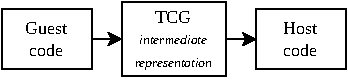
\includegraphics[height=70px]{figures/Translation_Guest-TCG-Host.pdf}
	\caption{TCG translation process}
\end{figure}

\noindent
The translation process is twofold, first phase consists of translating the guest code, for example a RISC-V compiled
workload, to an \textbf{TCG Intermediate Representation} (referred to as \textit{TCG IR}), this part is
called \textit{The frontend}. The second phase translates the TCG IR to the host ISA code, this part is called
\textit{The backend}.%
\footnote{Such notion of the backend and frontend operations allows the simulator to separate the adaptation
of new guest and host architectures, making the simulator more flexible.}

The following sections will only explain the basics of both TCG operations, as these mechanisms are very
complicated. Note that this flow only happens when there is no cached Translation Block found. The topic of TBs and
their caching will be explained later, for now, we only care about the code translation mechanisms.

\subsection{Main execution loop}

The main CPU execution method, \texttt{cpu\_exec()}, tries to find a cached translation block using
\texttt{tb\_find\_fast()}, if this fails the \texttt{tb\_find\_slow()} is called. If a block is found, the host starts
executing the translated code. If this function does not find the block, the \texttt{tb\_gen\_code()} is called.
This function allocates memory for a to-be-created translation block and sets needed flags in it. After that is done,
the \texttt{cpu\_gen\_code()} is called:

\nopagebreak[4]
\begin{lstlisting}[
    style=lstC,
    label={lst:cpu-gen-code},
    caption={The \texttt{cpu\_gen\_code()} code. Variable declaration omitted.}
    ]
void cpu_gen_code(CPUState *env, TranslationBlock *tb, ...)
{
    tcg_func_start(s);
    cpu_gen_code_inner(env, tb);

    /* generate machine code */
    gen_code_buf = tb->tc_ptr;
    tb->tb_next_offset[0] = 0xffff;   tb->tb_next_offset[1] = 0xffff;

    s->tb_next_offset = tb->tb_next_offset;
    s->tb_jmp_offset = tb->tb_jmp_offset;
    s->tb_next = NULL;

    gen_code_size = tcg_gen_code(s, gen_code_buf);
    *gen_code_size_ptr = gen_code_size;

    search_size = encode_search(tb, gen_code_buf + gen_code_size);
    *search_size_ptr = search_size;
}
\end{lstlisting}

\subsection{TCG frontend}
\label{sec:tcg-frontend}

The first two calls from the code (\ref{lst:cpu-gen-code}), are responsible for generating an intermediate
representation. The \texttt{tcg\_func\_start()} initializes TCG, while the \texttt{cpu\_gen\_code\_inner()} prepares
\textit{DisasContext},%
\footnote{A DisasContext typically includes information such as the address of the machine code being disassembled,
the size of the code, and the type of CPU architecture the code is intended for. It may also include pointers to other
data structures or functions that are used by the disassembler}
and starts a translation loop.

The main part of the translation loop is the \texttt{gen\_intermediate\_code()} call, this is a platform-specific
IR generation method. This function later calls the \texttt{disas\_insn()} routine, responsible for disassembling
the instruction, I.e. in the RISC-V implementation this function determines whether the type of opcode under the current
program counter (is it a compressed instruction? does the opcode belong to a custom extension?). After determining
the type of the opcode, the according decode function is called. Since we are considering RISC-V ISA, the decode function
is \texttt{decode\_RV32\_64G()}. The decode function then parses opcode according to the ISA standard, and calls a
function that will generate IR opcodes:

\begin{lstlisting}[
    style=lstC,
    label={lst:decode-rv32},
    caption={Opcode decoding on an example of RISC-V \texttt{addi}.}
    ]
static void decode_RV32_64G(CPUState *env, DisasContext *dc)
{
    op = MASK_OP_MAJOR(dc->opcode);
    rs1 = GET_RS1(dc->opcode);
    rs2 = GET_RS2(dc->opcode);
    rd = GET_RD(dc->opcode);
    imm = GET_IMM(dc->opcode);
    rm = GET_RM(dc->opcode);

    switch (op) {
        case OPC_RISC_ARITH_IMM:
        gen_arith_imm(dc, MASK_OP_ARITH_IMM(dc->opcode), rd, rs1, imm);
        break;
        ...
    }
}

static void gen_arith_imm(DisasContext *dc, uint32_t opc, int rd, int rs1, long imm)
{
    switch (opc) {
    case OPC_RISC_ADDI:
        tcg_gen_addi_tl(source1, source1, imm); //#define tcg_gen_addi_tl   tcg_gen_addi_i32
        break;
    ...
    }
}
\end{lstlisting}

\noindent
The translation loop continues indefinitely until one of the following conditions is met:
\begin{itemize}
    \item{Number of instructions in TB has reached a maximum allowed value, or an error occurred,}
    \item{There are breakpoints defined, and the breakpoint address matches the current PC,}
    \item{Last translated opcode is a jump instruction.}
\end{itemize}

\pagebreak
\subsection{TCG backend}

The rest of the function from (\ref{lst:cpu-gen-code}) is responsible for recompiling an IR to the host architecture.
The first part of the code prepares the translation block and can be skipped for now. The actual transition occurs
in the \texttt{tcg\_gen\_code()} function:

\begin{lstlisting}[
    style=lstC,
    label={lst:tcg-gen-code},
    caption={IR to host encoding.}
    ]
static inline int tcg_gen_code_common(TCGContext *s, uint8_t *gen_code_buf)
{
    for (;;) {
        opc = tcg->gen_opc_buf[op_index];
        def = &tcg_op_defs[opc];
        switch (opc) {
        case INDEX_op_movi_i32:
            tcg_reg_alloc_movi(s, args);
            break;
        ...
        case INDEX_op_call:
            dead_args = s->op_dead_args[op_index];
            args += tcg_reg_alloc_call(s, def, opc, args, dead_args);
            goto next;
        case INDEX_op_end:
            goto the_end;
        ...
        default:
            dead_args = s->op_dead_args[op_index];
            tcg_reg_alloc_op(s, def, opc, args, dead_args);
            break;
        }
    }
}
\end{lstlisting}

\noindent
This method handles special IR micro-ops first, such as exiting the block or calling a helper function (more about them
later). If the \texttt{opc} does not match any of the special cases, the code falls through to the \texttt{default}
block, where the \texttt{tcg\_reg\_alloc\_op()} is called, witch then calls target-specific \texttt{tcg\_out\_op()} method.

\begin{lstlisting}[
    style=lstC,
    label={lst:tcg-out-op},
    caption={Generating \textit{target} instructions from IR.}
    ]
static inline void tcg_out_op(TCGContext *s, TCGOpcode opc, const TCGArg *args, ...)
{
    switch(opc) {
        case INDEX_op_exit_tb:
            tcg_out_movi(s, TCG_TYPE_PTR, TCG_REG_EAX, args[0]);
            tcg_out_jmp(s, (tcg_target_long) tb_ret_addr);
            break;
        case INDEX_op_br:
            tcg_out_jxx(s, JCC_JMP, args[0], 0);
            break;
    }
}
\end{lstlisting}

\pagebreak
\subsection{Example of code translation using TCG}

The best way to illustrate the operations of TCG, is to provide an example, let's look at an example of RISC-V to IR to
x86 translation. This example comes from booting a Zephyr RTOS "Hello World" demo on a QEMU-RV32 system:%
\footnote{The QEMU flags to create such logs: \texttt{-d in\_asm, -d out\_asm, -d op}.}

\begin{itemize}
    \item{RISC-V guest machine code:
    \begin{lstlisting}[frame=tblr]
    0x00001000:  00000297          auipc           t0,0            # 0x1000
    0x00001004:  02828613          addi            a2,t0,40
    0x00001008:  f1402573          csrrs           a0,mhartid,zero
    \end{lstlisting}
    }
    %
    \item{TCG IR micro-ops:
    \begin{lstlisting}[frame=tblr, label={lst:tcg:tcgir-microops}]
    0x00001000:   mov_i32 x5/t0,$0x1000
    0x00001004:   add_i32 x12/a2,x5/t0,$0x28
    0x00001008:   mov_i32 tmp5,$0x1
                  st_i32 tmp5,env,$0xfffffffffffff1a8
                  call csrr,$0x0,$1,x10/a0,env,$0xf14
                  mov_i32 pc,$0x100c
                  exit_tb $0x0
                  set_label $L0
                  exit_tb $0x7fef28000043
    \end{lstlisting}
    }
    %
    \item{x86 host machine code:%
    \footnote{The \texttt{callq} opcode uses \textit{RIP Relative Adressing}, allowing the call location to be
    intermixed with the code. Using GDB it was possible to verify that \texttt{0x000055a84d2b8e00}
    was the addres of an according helper function.}
    \begin{lstlisting}[frame=tblr, label={lst:tcg:x86translated}]
    0x7eff7c000123:  c7 45 14 00 10 00 00           movl     $0x1000, 0x14(%rbp)
        -- guest addr 0x00001004
    0x7eff7c00012a:  c7 45 30 28 10 00 00           movl     $0x1028, 0x30(%rbp)
        -- guest addr 0x00001008
    0x7eff7c000131:  c7 85 a8 f1 ff ff 01 00        movl     $1, -0xe58(%rbp)
    0x7eff7c000139:  00 00
    0x7eff7c00013b:  48 8b fd                       movq     %rbp, %rdi
    0x7eff7c00013e:  be 14 0f 00 00                 movl     $0xf14, %esi
    0x7eff7c000143:  ff 15 1f 00 00 00              callq    *0x1f(%rip)
    0x7eff7c000149:  89 45 28                       movl     %eax, 0x28(%rbp)
    0x7eff7c00014c:  c7 85 18 12 00 00 0c 10        movl     $0x100c, 0x1218(%rbp)
    0x7eff7c000154:  00 00
    0x7eff7c000156:  e9 bb fe ff ff                 jmp      0x7eff7c000016
    0x7eff7c00015b:  48 8d 05 e1 fe ff ff           leaq     -0x11f(%rip), %rax
    0x7eff7c000162:  e9 b1 fe ff ff                 jmp      0x7eff7c000018
    ...
    data: [size=8]
    0x7eff7c000168:  .quad  0x000055a84d2b8e00
    \end{lstlisting}
    }
\end{itemize}

\noindent
The \textit{TB Prologues} have been omitted, as they will be covered in a section discussing the translation blocks.
Upon further inspection, one can notice that the guest \texttt{csrrs} opcode has emitted an host \texttt{call} opcode.
This brings us to the topic of helper functions.

\pagebreak
\subsection{Helper functions}

Helper functions serve the purpose of emulating incompatible instructions by delegating their execution to the
simulation layer, essentially bypassing the main TCG translation mechanisms. Examples of such functions include
architecture-specific instructions, for example, accessing guests' control and status registers, and memory access
instructions, which are handled by SoftMMU.

Helper functions are akin to the idea of callbacks or trampolines in higher-level programming languages. Helpers calls
are dynamically included in the TCG IR, when the opcode gets parsed in the decode function (for example in previously
mentioned (\ref{lst:decode-rv32})).

These are not called directly in code, both Tlibs and QEMU implement helper generation evil pre-processor macros.


\begin{lstlisting}[
    style=lstC,
    label={lst:csrrs-helper},
    caption={RISC-V \texttt{csrrs} helper.}
    ]
target_ulong helper_csrrs(CPUState *env, target_ulong src, target_ulong csr, target_ulong rs1_pass)
{
    validate_csr(env, csr, rs1_pass != 0);
    uint64_t csr_backup = csr_read_helper(env, csr);
    if (rs1_pass != 0) {
        csr_write_helper(env, src | csr_backup, csr);
    }
    return csr_backup;
}
\end{lstlisting}

\section{Translation Blocks}

The previously described translation process may seem overly convoluted, but when paired with the ability to cache and
reuse translated code, it significantly enhances the overall performance of the simulator. This is immensely important
in this context, as speed is one of the main distinguishing features of QEMU and Tlib.

Building up upon the knowledge from the previous section, when TCG is translating the code, it divides the
code into the \textbf{smallest possible standalone pieces of code}, by this, we understand the code that has only one
possible exit point. In other words, translation blocks always end on:
\begin{itemize}
    \item{Branching instructions, including both conditional and unconditional jumps, calls, and returns.}
    \item{Helper callbacks, because they call an external code, the TB execution must be halted. This can be seen
    in the TCG IR micro-ops (\ref{lst:tcg:tcgir-microops}) example, where the \texttt{tb\_exit} micro-op is emitted
    after an \texttt{csrrs} helper was called.}
\end{itemize}

In the case of conditional branches, the QEMU and Tlibs implement a \textit{Lazy evaluation of the CPU condition codes},
as in, the TCG only translates one path of the branching instruction. If the TCG were to generate native machine code
for both the taken and not-taken paths of the branch, it would have to generate twice as much machine code as is needed.
By using lazy evaluation, the TCG can generate the native machine code for the taken path of the branch only when the
branch is taken, rather than generating machine code for both paths in advance \cite{QemuInternalsTech}.

\pagebreak
\begin{figure}[h]
	\centering
	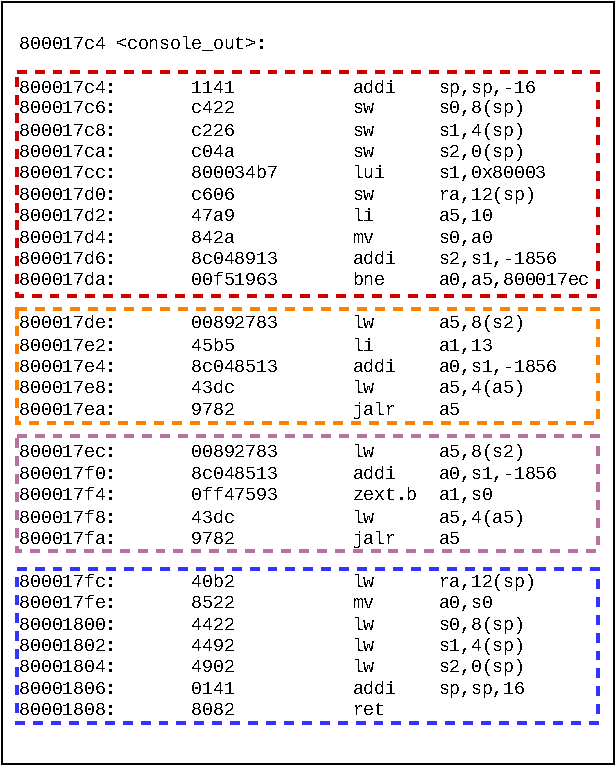
\includegraphics[height=400px]{figures/TranslactionBlocks.pdf}
	\caption{An example of basic block division.}
    \label{fig:block-division}
\end{figure}

\subsection{Translation Block caching}

After each block translation, the translated block is appended to the \textbf{TCG Translation Block Cache}.
The QEMU Internals, states that "A 32 MByte cache holds the most recently used translations. For simplicity, it is
completely flushed when it is full" \cite{QemuInternalsTech}. The cache also needs to be flushed when the code modifies
itself, this is accomplished by setting a host memory page holding the code to be read-only. Then if the
write-protected region is modified, the Linux will emit a \texttt{SEGV} signal, that will be handled by QEMU. This
invalidates and flushes the cache, as well as flushes direct block chaining lists.

This feature significantly improves the performance of the simulator, as the code usually needs to be translated only
once, significantly reducing the simulation overhead. This optimization also enables another performance improvement,
that aims to mitigate the performance penalty needed for the context switch between the translated guest code and the
QEMU runtime. This will be described in the next section.

\pagebreak
\subsection[Translation Block chaining]{Translation Block chaining
\footnote{A notable portion of the images in this section was inspired by Chad D. Kersey's presentation
\cite{QemuInternalsPresentation}.}}

Block chaining is a technique used to reduce the time spent on context switching between translated guest code and the
runtime of the simulator. The majority of the context switch time comes from the fact that the CPU state, such as
registers and status flags, has to be saved into memory. Memory operations and context swaps tend to be
the slowest things a CPU does, as they might require up to a hundred cycles.
% mabye put some google scheduler slides idk?

\subsection*{No block chaining}

Assuming there is no block chaining, each block execution will look like this:
\begin{figure}[h]
	\centering
	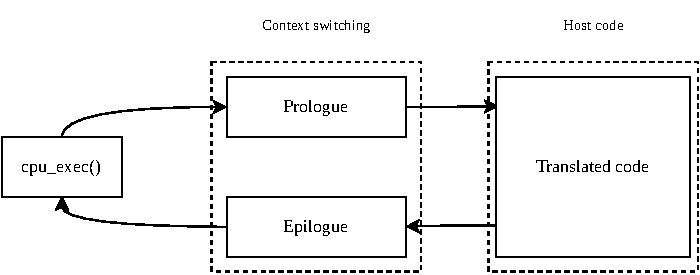
\includegraphics[width=0.75\textwidth]{figures/TbExecution-NoChain.pdf}
	\caption{Execution flow with no block chaining}
\end{figure}

\noindent
The \textit{Context switching} block consists of two elements, a \textit{Prologue} and an \textit{Epilogue}. The former
saves the Runtime context, swaps the previously saved context to the host code execution, and jumps to the code pointer.
The latter saves the host code execution context, restores the simulator runtime context, and jumps to the
\texttt{cpu\_exec()} loop.
Looking at the example Translation Blocks from Fig. (\ref{fig:block-division}), one might notice that returning to a
main loop after each block execution will cause a lot of context switching, which would be a huge detriment to the
overall performance of the simulator.

\subsection*{Direct block chaining}

To mitigate this issue, the QEMU developers came up with a mechanism, that chains the block execution. This allows the
simulator to directly link each block with another, greatly reducing the overhead from context swapping.
This comes at the price of increased code complexity and additional possible issues stemming from the
self-modifying code, with the latter being especially prevalent in the SMP system emulation.

This is accomplished by leaving extra space in a translated code, just before a return to the epilogue. Later, when
the code is finished executing and has not been patched to jump to any other TB, the block returns to the epilogue,
in turn, exits to the \texttt{cpu\_exec()}. The main loop then tries to chain this block, to the next block. This
process is repeated for every exiting block.

There are other ways to chain TB that do not require exiting the host code, instead, these methods are executed at the
translation phase of the code. These mechanisms are explained in detail in the QEMU Translator Internals documentation,
at the Direct block chaining section \cite{QemuDocsChaining}.

\pagebreak

\begin{figure}[h]
	\centering
    \label{fig:qemu-execution-with-blocks}
	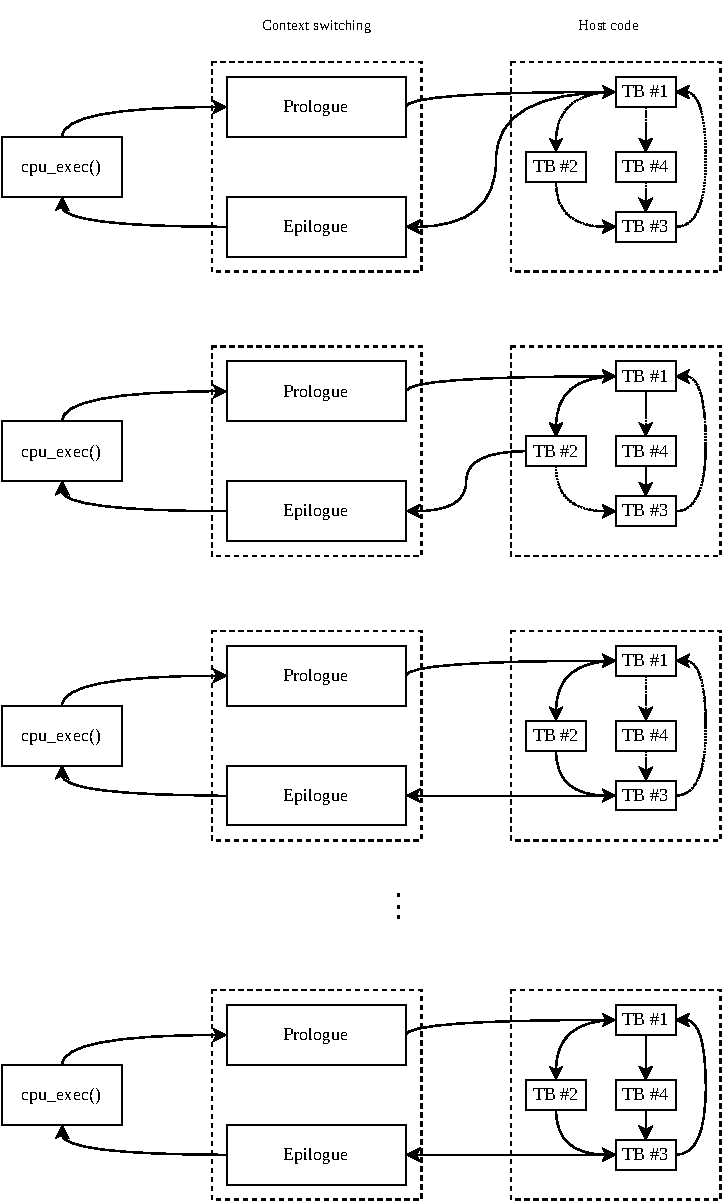
\includegraphics[width=0.7\textwidth]{figures/TbExecution-Chain.pdf}
	\caption{Execution flow with block chaining}
\end{figure}

\noindent
This relatively simple mechanism can create high-speed execution loops, even to the point where the host code
might not exit a loop for a very long time.

This is an interesting case, because such behavior can be classified as
blocking, and might be an issue when dealing with asynchronous interrupts. Let's assume that the binary doesn't fill up
the whole transition cache, the code never overwrites itself, and the TBs have been patched in a way that creates a
loop. In such cases, handling asynchronous exceptions is not possible, as the code never exits back to the main loop.

This problem has been solved by adding another thread, that is polling for interrupts, and if one is received, the
simulator will invalidate all of the TB's chains, exiting to the main loop at the end of the current TB.

\pagebreak

\section{Code Execution}

In the final section of this chapter, we will examine various issues and questions that may arise during the execution
of translated code.

\subsection{Staring the execution of the translated code}

When the simulator finds the Translation Block it executes the \texttt{tcg\_tb\_exec()} function, which is a
macro-definition, which casts a translation buffer to a function pointer, then calls it with arguments.

\begin{lstlisting}[
    style=lstC,
    caption={Executing the translation buffer.}
    ]
int cpu_exec(CPUState *env)
{
    ...
    env->current_tb = tb;
    asm volatile ("" ::: "memory");
    if (likely(!env->exit_request)) {
        tc_ptr = tb->tc_ptr;
        /* execute the generated code */
        next_tb = tcg_tb_exec(env, tc_ptr);
    }
    ...
}

#if !defined(tcg_tb_exec)
#define tcg_tb_exec(env, tb_ptr) \
    ((uintptr_t REGPARM (*)(void *, void *))tcg->code_gen_prologue)(env, tb_ptr)
#endif
\end{lstlisting}

\subsection{Exception and interrupt handling}

Exceptions and interrupts are an inseparable part of the CPU simulation, without them, the CPU would not be able to
handle most workloads. The logic handling them is fully architecture dependent, but this section will cover the
generic code. All of the examples are shown using a RISC-V instruction set.

By exception, we understand an event that occurs from the CPU itself. These events might happen upon user request, such
as \texttt{ecall} instruction or they might happen spontaneously, for example, a \texttt{mbadaddr} condition.

The term interrupts, often referred to as asynchronous exceptions, are a result of an external device sending an
interrupt request (\textit{IRQ}) to the CPU. An example of such an event is an External Timer sending an interrupt that
compares time has been reached, or a network device to signal that a new packet is ready to be handled.

\pagebreak
\subsection*{Exception generating}
The exceptions are generated using the beforementioned helper functions:

\begin{lstlisting}[
    style=lstC,
    caption={Generating exceptions using handlers.}
    ]
static inline void __attribute__ ((__noreturn__))
do_raise_exception_err(CPUState *env, uint32_t excpt, uintptr_t pc, uint32_t call_hook)
{
    env->exception_index = excpt;
    cpu_loop_exit_restore(env, pc, call_hook);
}

...

void helper_raise_exception_mbadaddr(CPUState *env, uint32_t excpt, target_ulong bad_pc)
{
    env->badaddr = bad_pc;
    do_raise_exception_err(env, excpt, 0, 1);
}
\end{lstlisting}

\subsection*{Interrupt generating}
The interrupts are generated in a different flow. A virtual device can \textit{send} an interrupt, by setting the
\texttt{exception\_index} to a value matching the ISA standards. The rest of the flow is identical to the exception
handling.

In the case of the QEMU, the interrupts are handled by the QEMU system module. In Renode's Tlibs, the external
interrupts are sent from the Renode framework, in this scenario extra care needs to be put in when dealing with
interrupt requests, such as using atomic operations, using locks on variables, etc.

\subsection*{Handling the exceptions in the main loop}

The main loop makes use of C library \texttt{setjmp/longjmp} for exception handling inside the simulated CPU.
The \texttt{setjmp} env is set just before the main execution loop. If the exception occurs the execution loop handles
the exception, then using \texttt{longjmp} jumps back to the point before an event occurred. This implementation allows
the CPU thread to exit deep and complex TCG translation functions.

It is worth noting that exceptions and interrupts are handled by the same function, the only aspect where they are
different is a way, in which the event is generated.

\pagebreak

\begin{lstlisting}[
    style=lstC,
    caption={Handling exceptions in the main loop.}
    ]
int cpu_exec(CPUState *env)
{
    env->exception_index = -1;
    /* before TB execution */
    for (;;) {
        if (setjmp(env->jmp_env) == 0) {
            if (env->exception_index >= EXCP_INTERRUPT) {
                ret = env->exception_index;
                // An event is an exception, not an interrupt
                // Skip to the second for loop, and handle it there
                break;
            } else {
                do_interrupt(env);
            }
        }
        ...
        /* TC execution */
        for(;;)
        {
            if (unlikely(env->exception_index != -1)) {
                cpu_loop_exit_without_hook(env);
            }
        }
    ...
\end{lstlisting}

\noindent
The events are then handled in the architecture specific \texttt{do\_interrupt()} function:

\begin{lstlisting}[
    style=lstC,
    caption={Generating interrupts using \texttt{do\_interrupt()}.}
    ]
void do_interrupt(CPUState *env)
{
    if (env->nmi_pending > NMI_NONE) {
        do_nmi(env);
        return;
    }
    if (env->exception_index == EXCP_NONE) {
        return;
    }
    ...
    if (env->priv == PRV_M || !((is_interrupt ? env->mideleg : env->medeleg) & (1 << bit))) {
    /* handle the trap in M-mode */
    env->mepc = env->pc;
    env->mcause = fixed_cause;
    if (hasbadaddr) {
        env->mtval = env->badaddr;
    }
    ...
}
\end{lstlisting}
